% The Bridge Experiment — final report, LaTeX edition.
% Source of truth: docs/research/BRIDGE-REPORT.md (converted 2026-07-25).
% Figures: figures/fig*.pdf, generated from benchmark data by
% recompute_figdata.py + generate_figures.py (every plotted value asserted
% against the markdown report).
% Build: latexmk -pdf report.tex
\documentclass[10pt]{article}

\usepackage[margin=1in]{geometry}
\usepackage[T1]{fontenc}
\usepackage[utf8]{inputenc}
\usepackage{lmodern}
\usepackage{microtype}
\usepackage{booktabs}
\usepackage{graphicx}
\usepackage{amsmath,amssymb}
\usepackage{array}
\usepackage{enumitem}
\usepackage[hidelinks]{hyperref}
\urlstyle{tt}

\setlist{itemsep=2pt,topsep=3pt,parsep=0pt}
\setlength{\emergencystretch}{2.5em}
\tolerance=2000
\newcommand{\code}[1]{\texttt{#1}}
\newcommand{\best}[1]{\textbf{#1}}

\title{\textbf{The Bridge Experiment: Does an Informal$\leftrightarrow$Formal
Join Move End-Task Lean Performance?}}
\author{Jack McCarthy\\
\normalsize WikiLean \,$\cdot$\, \url{https://wikilean.jackmccarthy.org}\\
\normalsize with experiments executed by Claude Code agents under direction}
\date{Final report --- July 25, 2026}

\begin{document}
\maketitle

\begin{center}
\begin{minipage}{0.92\textwidth}
\small
Preregistration: \code{docs/research/BRIDGE-EXPERIMENT.md},\\
commit \code{0d36f2664ab2ebb2c7b80b350d3c9bd820414335} (2026-07-16).\\[2pt]
Results log: \code{docs/research/BRIDGE-RESULTS.md}. All data, code, and run
transcripts are preserved in the private repository
\code{Deicyde/wikilean-bridge-experiment} (file map in
Section~\ref{sec:data}). Every number below is recomputable from a file in
that repository; the file is named where each table appears.
\end{minipage}
\end{center}

\section{Abstract}\label{sec:abstract}

We test whether making the informal$\leftrightarrow$formal join easy --- a
curated dictionary between mathematical concepts and Mathlib declarations
(the WikiLean ``Brain''), as opposed to mere access to both corpora ---
improves language-model performance on formalization tasks. Five
preregistered arms isolate the join: no tools (A), informal search (B),
formal search (C), the joined bridge (D), and both corpora side by side but
unjoined (E). Grading is mechanical throughout, and typechecking alone never
counts as success. We report three headline results. First, on 100
contamination-proof tasks built from Mathlib theorems newer than every
index, the bridge arm reaches 42\% folded success against 16\% for the
unjoined-tools control (McNemar 32 vs.\ 6 discordant, exact $p < 0.0001$),
while the no-tool arm collapses from 59.6\% to 20\%, which puts a number on
ProofNet memorization; the bridge also cuts hallucinated-decl citations to
6.8\%, against 17.7--26.3\% in every other arm. Second, on third-party
retrieval gold (MathlibQR-810, MathlibMPR), a Sonnet agent given the union
of bridge and formal-search tools, plus a manual distilled from measured
tool behavior, sets the best rows we know of on both benchmarks (R@10
0.885; group-recall@10 0.557 against the specialist SOTA of 0.461). Third,
the join does not help premise selection (0.272 vs.\ 0.453 for formal
search); this is the concept$\neq$premise boundary we preregistered, now
quantified as an 18pp API target.

\section{The system under test: the WikiLean Brain}\label{sec:system}

The artifact everything below measures is the WikiLean ``Brain'': a curated
knowledge graph over mathematics that joins Wikipedia/Wikidata concepts,
Mathlib4 declarations, and the external mathematical databases (nLab,
LMFDB, the Stacks project, ProofWiki, and others) into one map. Its atom is
a \emph{cell}: when a Lean declaration, a Wikidata concept, an encyclopedia
article, and a database page all denote the same mathematical object, they
are \emph{organs} of one cell rather than separate nodes --- Mathlib's
\code{Module}, Wikidata's ``module'' \emph{and} its ``vector space'' are a
single atom, because Mathlib has no \code{VectorSpace}; \code{Module}
generalizes it. Mathlib's folder hierarchy supplies the containment
altitude, and everything known about a cell (Lean source, descriptions,
licensed database snippets) is embedded on the cell itself. About 12{,}000
of Mathlib's declarations are concept-joined this way; the Brain is a map
of Mathlib, not the territory.

Agents reach it through an MCP server (\code{POST /mcp} on the live site)
exposing eight tools. \code{brain\_bridge} is the informal$\to$formal entry
point: free text in, existence-verified declarations out, each with its
signature, import line, and bond quality. \code{brain\_search} resolves
labels and aliases to atoms; \code{brain\_cell} returns the full atom card;
\code{brain\_transfer} makes the one-atom informal$\leftrightarrow$formal
jump; \code{brain\_neighborhood} walks the synapse graph;
\code{brain\_snippets} and \code{brain\_filter} serve stored content and
facet queries. The eighth, \code{decl\_exists}, is different in kind: a
batch existence check against the full declaration index --- all of
Mathlib, not just the joined subset --- built to be called on every name an
agent is about to cite.

Why build such a thing? The working hypothesis behind WikiLean is that
informal mathematics (what things are called and mean) and formal
mathematics (what typechecks) are two corpora whose \emph{join} is the
scarce artifact: a language model already holds both corpora loosely, and
the informal$\leftrightarrow$formal boundary is precisely where its
hallucinations live. If that is right, then curating the join --- names
verified, concepts merged, bonds carrying provenance --- should move
performance on end tasks, not just on lookup. Whether it actually does is
the question this report answers.

\section{Hypothesis and preregistered design}\label{sec:design}

\paragraph{Hypothesis (operationalized).} Since ``necessary'' is unprovable,
the preregistration commits to three predictions. P1: an agent with the
\emph{joined} dictionary beats an agent given informal and formal search
\emph{separately} --- if D $>$ E, then the join, not corpus access, carries
the effect. P2: the bridge solves at lower cost. P3: the bridge lifts
grounding (fewer hallucinated declaration citations), not just compile rate.

\paragraph{The five arms.} All five arms share the same model, prompt, and
budgets within each phase; the only thing that differs between them is the
tool manifest (\code{bench/run\_bridge.py}, manifests in \code{bench/arms/});
see Table~\ref{tab:arms}.

\begin{table}[htbp]
\centering
\small
\begin{tabular}{@{}lp{0.42\textwidth}p{0.27\textwidth}@{}}
\toprule
Arm & Tools & Isolates \\
\midrule
A \code{no\_tools} & none (\code{--tools ""}) & floor / memorization \\
B \code{informal} & Wikipedia + nLab search/fetch, no Lean mapping & informal reasoning alone \\
C \code{formal} & loogle + ripgrep + source read over pinned Mathlib & the LeanSearch-class status quo \\
D \code{wikibrain} & the Brain MCP (\code{brain\_bridge}\slash\code{search}\slash\code{cell}\slash\code{transfer}\slash\code{neighborhood}\slash\code{snippets}\slash\code{filter} + batch \code{decl\_exists}) & the join \\
E \code{B+C unjoined} & B's tools AND C's tools, no join & the decisive control \\
\bottomrule
\end{tabular}
\caption{The five preregistered arms. Identical model, prompt, and budgets;
only the tool manifest differs.}
\label{tab:arms}
\end{table}

{\sloppy
\paragraph{Models per phase.} Tier 1 (statement autoformalization) uses
\code{claude-haiku-4-5} (model id \code{claude-haiku-4-5-20251001}) in all
five arms. Bridge v2 (retrieval and proving) uses \code{claude-sonnet-5} in
all agent arms, per an explicit pre-execution decision
(\code{docs/research/BRIDGE-V2-BENCHMARKS.md}, 2026-07-25).\par}

\paragraph{Grading rules.} Typecheck is never success by itself;
TheoremGraph~\cite{theoremgraph} reports 22/24 outputs typechecking while
only 5/24 were correct. A Tier-1 run counts as a success only when it
produced a declaration, cited zero hallucinated names, and typechecks on the
pinned toolchain. We quarantined the preregistered LLM-judge faithfulness
leg behind a human-calibration gate and ultimately dropped it in favor of
graders that existed before the arms did --- third-party gold labels and the
Lean kernel; Section~\ref{sec:limitations} explains why. Hallucinated-decl
rate is graded against a union oracle (doc-gen4 declaration data $\cup$
verified renames; the extractor is documented in
\code{bench/score\_bridge.py}).

\paragraph{Task sets.} Tier 1a is ProofNet\#: 371 problems (341 eval plus 30
prompt-freezing dev, all scored), pinned to \code{PAug/ProofNetSharp}
@\code{a8da405fbd1e348a87445c2e562c747b7e26dc8f}
(MIT;~\cite{proofnetsharp}) and graded on Lean v4.32.0-rc1 / Mathlib
\code{a33a5ccd}. Tier 1b is 100 fresh tasks built from theorems merged into
Mathlib master between 2026-07-03 and 07-16, provably absent from every
arm's index including the Brain's decl universe
(\code{bench/data/fresh\_tasks.stats.json} records the held-out guarantee);
these are graded on Lean v4.33.0-rc1 / Mathlib \code{9944fe29}. A second
independent determinacy annotation (agreement 79\%, $\kappa \approx 0.20$;
the annotators apply complementary strictness) defines a 74-task
both-determinate primary subset.

\paragraph{Budgets.} Every arm ran under the same budget: 30 turns stated in
the prompt and a 10-minute wall clock, enforced. Agents had no in-loop
typechecker and were instructed to verify cited names through their tools.

\paragraph{Protocol deviations} (recorded in the preregistration before any
result existed; numbering as in that document):

\begin{enumerate}
\item The turn budget is prompt-stated and wall-clock-enforced (the CLI
  lacks \code{--max-turns}); turns are recorded per row.
\item Arm D talks to the production Worker code served locally over the
  shipped shard bytes (\code{bench/arms/local\_worker.mts}), with snapshot
  pins echoed per response.
\item Grading uses a persistent REPL (Mathlib loaded once) rather than
  single-shot elaboration, on the same pins.
\item Agents had no in-loop typechecking this campaign, which makes
  hallucinated-decl rate a pure grounding measure.
\item Judge grades were excluded from all claims pending human calibration
  (subsequently superseded by the v2 judge-free design).
\item \textbf{Skill-leak seal (deviation 6).} The dev smoke showed tool arms
  B--E calling the CLI's built-in \code{Skill}/\code{ToolSearch} (32--56
  calls/arm) and loading, for example, Mathlib-conventions text that arm A
  structurally could not reach --- an asymmetric contamination. We added
  \code{Skill}, \code{ToolSearch}, and \code{Agent} to the disallowed-tools
  list \emph{before any eval run}, quarantined the 120 contaminated B--E dev
  runs unscored to \code{bench/data/runs\_devleak\_2026-07-18/}, and re-ran
  them clean.
\item \textbf{Trace telemetry (deviation 7).} From eval arm C onward we
  retained per-call tool traces (truncated input, result head, error flag),
  observation-only --- nothing any agent sees changed. As a consequence,
  eval arms C/D/E and all fresh runs carry traces; eval A/B carry
  name-counts only.
\end{enumerate}

\section{Tier 1: statement autoformalization (claude-haiku-4-5)}\label{sec:tier1}

\subsection{Tier 1a --- ProofNet\# ($n=371$/arm)}\label{sec:tier1a}

The source is \code{docs/research/BRIDGE-RESULTS.md}, and every number is
recomputable from \code{bench/data/bridge\_summary.json} plus
\code{bench/data/runs/}. Success requires a produced declaration, no
hallucinated citation, and a passing typecheck. Results in
Table~\ref{tab:tier1a}.

\begin{table}[htbp]
\centering
\small
\begin{tabular}{@{}lccccc@{}}
\toprule
metric & A none & B wiki & C formal & D wikibrain & E B+C unjoined \\
\midrule
success (folded) & 59.6\% & 57.1\% & 62.3\% & \best{64.2\%}$^{a}$ & 60.9\% \\
success\_proxy (no-halluc) & 76.8\% & 72.8\% & 72.2\% & \best{84.6\%} & 71.2\% \\
typecheck ok & 66.6\% & 63.6\% & 81.9\% & 74.7\% & \best{83.3\%} \\
halluc-decl rate & 10.1\% & 11.0\% & 10.6\%$^{a}$ & \best{5.9\%} & 11.3\% \\
runs w/ hallucination & 86 & 101 & 103 & \best{57} & 107 \\
\bottomrule
\multicolumn{6}{@{}p{0.94\textwidth}@{}}{\footnotesize $^{a}$\,Corrected for
display rounding relative to the markdown report and results log, which
printed D success 64.1\% and C halluc-decl rate 10.7\%: the exact recomputed
values are $238/371 = 64.15\%$ and $140/1315 = 10.65\%$. No claim is
affected.} \\
\end{tabular}
\caption{Tier 1a --- ProofNet\# ($n=371$/arm). Bold marks the best column
per row.}
\label{tab:tier1a}
\end{table}

The preregistered McNemar test of D against E gives 63 vs.\ 51 discordant
pairs, exact $p = 0.30$: the direction favors D, but the test is
underpowered at this effect size. Two other readings matter. Arm A scoring
59.6\% with zero tools is substantial ProofNet memorization, and was the
motivation for Tier 1b. And the typecheck row \emph{anti-correlates} with
grounding --- E leads on typecheck (83.3\%) while trailing on
hallucinations, reproducing TheoremGraph's typecheck-is-not-a-signal
finding at $15\times$ their $n$.

\subsection{Tier 1b --- the fresh set ($n=100$/arm, contamination-proof)}\label{sec:tier1b}

Same files, restricted to the fresh tasks. With memorization stripped, the
field reorders (Table~\ref{tab:tier1b}, Figures~\ref{fig:success}
and~\ref{fig:halluc}).

\begin{table}[htbp]
\centering
\small
\begin{tabular}{@{}lccccc@{}}
\toprule
metric & A none & B wiki & C formal & D wikibrain & E B+C unjoined \\
\midrule
success (folded) & 20\% & 22\% & 25\% & \best{42\%} & 16\% \\
halluc-decl rate & 21.2\% & 17.7\% & 20.9\% & \best{6.8\%} & 26.3\% \\
runs w/ hallucination & 54 & 48 & 49 & \best{23} & 36 \\
\bottomrule
\end{tabular}
\caption{Tier 1b --- the fresh set ($n=100$/arm), built from Mathlib
theorems newer than every arm's index.}
\label{tab:tier1b}
\end{table}

\begin{figure}[htbp]
\centering
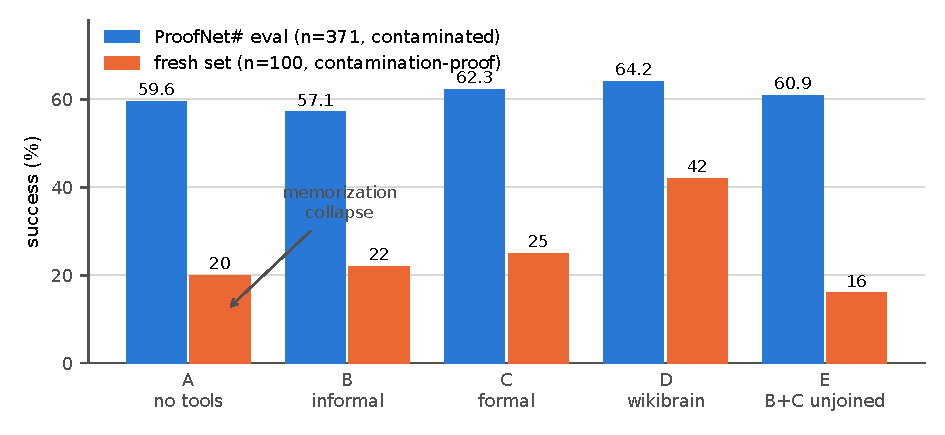
\includegraphics[width=\textwidth]{figures/fig1_tier1_success}
\caption{Tier-1 folded success by arm, ProofNet\# eval versus the
contamination-proof fresh set. Off-distribution, the no-tool arm collapses
$59.6\% \to 20\%$ while the bridge arm (D) holds 42\% against 16\% for the
unjoined-tools control (E). Data:
\code{bench/data/bridge\_summary.json} (paired matrix, split by task id).}
\label{fig:success}
\end{figure}

\begin{figure}[htbp]
\centering
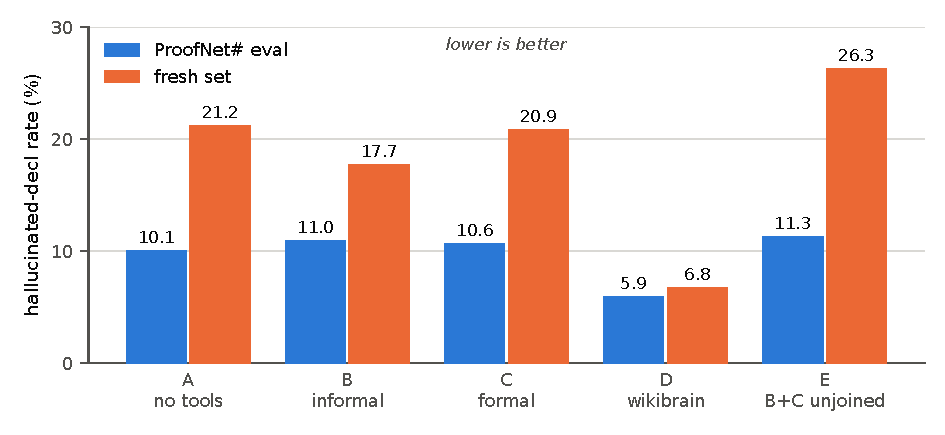
\includegraphics[width=\textwidth]{figures/fig2_halluc}
\caption{Hallucinated-declaration citation rate by arm (share of cited
declaration names absent from the union oracle). D's grounding advantage
\emph{widens} off-distribution: 6.8\% on the fresh set versus
17.7--26.3\% for every other arm. Data: recount over
\code{bench/data/runs/} with the \code{bench/score\_bridge.py} extractor
and oracle.}
\label{fig:halluc}
\end{figure}

Here the preregistered hypothesis test is decisive. McNemar D-vs-E gives
\textbf{32 vs.\ 6 discordant pairs, exact $p = 2.4\times10^{-5}$}; D-vs-C
gives 28 vs.\ 11 ($p = 0.0095$) and D-vs-A 29 vs.\ 7 ($p = 0.0003$). On the
held-out set it is the \emph{join} that carries the effect, not tool
volume. The result also survives restriction to the 74-task
both-determinate primary subset (recomputed from the
\code{bench/data/fresh\_tasks.jsonl} det fields crossed with the paired
matrix): D solves 31/74 (41.9\%) against E's 14/74 (18.9\%), McNemar 22
vs.\ 5, exact $p = 0.0015$, so the effect is not an artifact of
underdetermined prompts.

Three secondary observations. Arm A collapses from 59.6\% to 20\%
off-distribution, which quantifies the memorization. D's hallucination
advantage \emph{widens} off-distribution (6.8\% vs.\ 17.7--26.3\%). And arm
E is the worst arm at 16\%, producing no declaration at all in 31 of its
100 fresh runs --- unjoined tool volume can be actively harmful.

Cost tells the same story (recomputed from run rows; mean per task, folded
over all 471 runs/arm): A \$0.034, B \$0.048, C \$0.140, \best{D \$0.121},
E \$0.128, with mean wall-clock C 116\,s, D 89\,s, E 106\,s. The bridge arm
outscores the cheaper-per-task C and E while costing less than either, so
P2 holds directionally.

\subsection{Trace attribution (deviation-7 telemetry, eval C/D/E)}\label{sec:trace}

The traces (\code{bench/trace\_analysis.py} over \code{bench/data/runs/},
eval split) let us ask where cited names actually came from. Between 98\%
and 100\% of traced tool-arm runs cite at least one declaration that
visibly surfaced in a tool result, and only 10--17\% of citations never
touched the tools. In arm D, \textbf{35\% of runs (116/329) cite a
declaration that came out of a \code{brain\_bridge} /
\code{brain\_transfer} result} --- English in, formal name out --- and this
is an undercount, since result heads truncate at 200 chars. The sharpest
signal is among \emph{hallucinated} citations: the checked-and-cited-anyway
rate is 35\% for C and 30\% for E but only \textbf{13\% for D}. Binary
\code{decl\_exists} verification disciplines the model where the fuzzy
search neighborhoods of loogle and grep let it fool itself. This is the
mechanism behind the hallucination rows above.

\section{Third-party retrieval: MathlibQR-810 and MathlibMPR
(claude-sonnet-5)}\label{sec:retrieval}

Tier-1's remaining faithfulness leg depended on an LLM judge whose error
could correlate with arm, so Bridge v2 replaces judge-dependent grading
with graders that predate the arms: third-party expert gold labels here,
and the Lean kernel in Section~\ref{sec:sorrydb}. The data come from
\code{frenzymath/LeanSearch-v2} @\code{94f4888cbaf9} (CC BY 4.0;
LeanSearch-v2~\cite{leansearchv2}), copied under \code{bench/v2/data/}.
There are four arms: N (no tools), F (\code{loogle} + \code{decl\_grep} +
\code{decl\_read}), W (the Brain MCP), and WF (W $\cup$ F \textbf{plus}
\code{bench/v2/AGENT\_MANUAL.md} prepended to the prompt --- the manual is
deliberately part of the condition; see the confound note below). Scoring
is \code{bench/v2/score\_retrieval.py}, exact full-name match only; run
rows with full gzipped stream-json transcripts live in
\code{bench/v2/runs/agent/}.

\subsection{MathlibQR fair-810 --- concept retrieval (810 expert query rows,
6 styles)}\label{sec:qr}

\begin{table}[htbp]
\centering
\small
\begin{tabular}{@{}lcc@{}}
\toprule
system & R@10 & nDCG@10 \\
\midrule
published: TheoremGraph & 0.775 & 0.548 \\
published: LSv2 retriever+reranker & 0.780 & 0.623 \\
system-mode wikibrain (one \code{brain\_bridge} call, no LLM) & 0.036 & 0.031 \\
agent N & 0.633 & 0.598 \\
agent F & 0.831 & 0.790 \\
agent W & 0.816 & 0.781 \\
\best{agent WF} & \best{0.885} & \best{0.839} \\
\bottomrule
\end{tabular}
\caption{MathlibQR fair-810 concept retrieval. Exact full-name match; gold
is one declaration per query row.}
\label{tab:qr}
\end{table}

\begin{figure}[htbp]
\centering
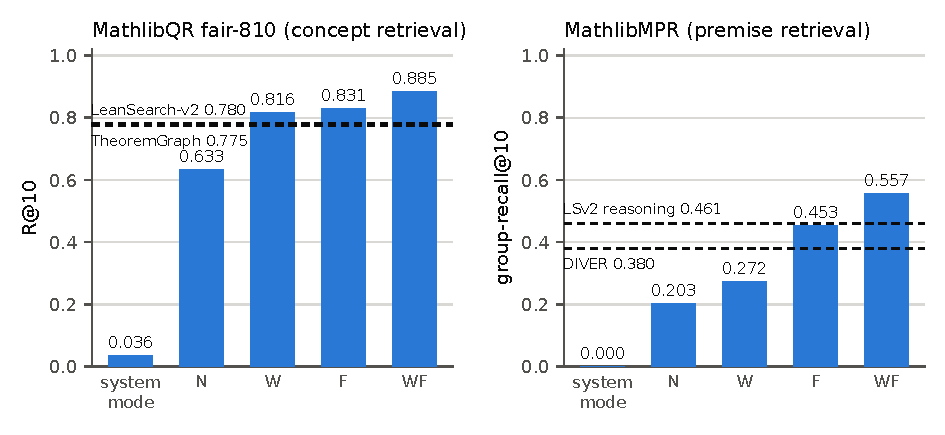
\includegraphics[width=\textwidth]{figures/fig3_retrieval}
\caption{Retrieval by system, with published anchors as dashed reference
lines. Left: MathlibQR fair-810 R@10 (anchors: TheoremGraph 0.775,
LeanSearch-v2 retriever+reranker 0.780). Right: MathlibMPR
group-recall@10 (anchors: LeanSearch-v2 reasoning 0.461, DIVER 0.380).
System-mode is a single \code{brain\_bridge} call with no LLM; N/W/F/WF are
Sonnet agent arms. Data: rerun of \code{bench/v2/score\_retrieval.py}.}
\label{fig:retrieval}
\end{figure}

The first thing Table~\ref{tab:qr} shows is a deficiency. System mode ---
one \code{brain\_bridge} call, no LLM --- scores 0.036, because the API's
free-text entry is a label/alias resolver, not a semantic retriever:
nickname queries reach nDCG 0.196 while the descriptive styles (LaTeX,
natural-language, special-case) score 0.000. Yet an agent \emph{iterating}
over the same API reaches 0.816. The content is in the graph; the
single-shot entry point is the gap. This is the headline API deficiency.

Among the agent arms, F and W are statistically tied (paired discordants 78
F-only vs.\ 66 W-only, exact $p = 0.36$), and both land nominally above the
published retriever rows --- with the apples-to-oranges caveat that agents
reason and verify while retrievers embed once
(Section~\ref{sec:limitations}). The two toolkits have different textures:
W wins the special\_case style (nDCG 0.523 vs.\ F's 0.384 --- the Brain's
curated special\_case bonds are the signal), while F wins the Lean-syntax
styles. Grep cannot find what source text never names.

WF is decisive. It beats F (71 vs.\ 27 discordant, exact
$p = 1.0\times10^{-5}$) and W (83 vs.\ 27, $p = 8.3\times10^{-8}$), and
sits +10.5pp R@10 above the best published retriever row. The style spread
narrows as well: every style reaches $\geq 0.55$ nDCG, and five of six
reach $\geq 0.81$. Agent N's 0.633, by contrast, includes 143/810 rows
scored 0 for format non-compliance (no JSON array in the final message), an
agent-mode failure the manual explicitly addresses.

The tool census: F averages 2.2 calls/run and W 3.5 (\code{decl\_exists}
1{,}251 + \code{brain\_bridge} 608 --- a verify-then-cite pattern), while
WF averages 4.6 calls pooled across both benchmarks in a genuine
dual-toolkit mix (\code{decl\_grep} ${\sim}1.5$k, \code{decl\_exists}
${\sim}0.9$k, \code{brain\_bridge} ${\sim}0.7$k, \code{decl\_read}
${\sim}0.5$k, \code{loogle} ${\sim}0.4$k). The \code{brain\_cell} misuse
pattern, a 63\% failure rate in the Tier-1 traces, disappears under the
manual. Figure~\ref{fig:tooluse} draws the whole census, SorryDB included.
Two compositional facts stand out: \code{decl\_exists} is the single
most-called tool wherever the Brain is present (1{,}473 calls in W ---
verify-then-cite made mechanical), and the manual does not so much add
tools as prune them --- WF keeps \code{brain\_bridge} as its informal entry
(687 calls) while \code{brain\_cell} falls from 482 calls in W to exactly
one.

\subsection{MathlibMPR --- premise retrieval (69 post-cutoff PR theorems,
expert premise groups)}\label{sec:mpr}

\begin{table}[htbp]
\centering
\small
\begin{tabular}{@{}lc@{}}
\toprule
system & group-recall@10 \\
\midrule
published: LeanSearch-v2 reasoning & 0.461 \\
published: DIVER & 0.380 \\
published: TheoremGraph concept-tuned & 0.165 \\
system-mode wikibrain & 0.000 \\
agent N & 0.203 \\
agent W & 0.272 \\
agent F & 0.453 \\
\best{agent WF} & \best{0.557} \\
\bottomrule
\end{tabular}
\caption{MathlibMPR premise retrieval: a group is covered when any of its
interchangeable members appears in the top 10.}
\label{tab:mpr}
\end{table}

Two results stand out. A generic Sonnet agent with grep and loogle
\textbf{matches the specialist premise retriever} (0.453 vs.\ 0.461), a
notable baseline result on its own. The Brain, by contrast, helps over
memory (+7pp) but trails formal search by 18pp: this is the preregistered
concept $\neq$ premise boundary (TheoremGraph's negative transfer), now
measured on our own tools, and it gives \code{brain\_premises}
(BRIDGE-ISSUES \#7) a quantified 18pp target. WF again beats both the best
single arm (+10pp over F) and the published SOTA on its own benchmark
(0.557 vs.\ 0.461).

\paragraph{The WF confound, stated plainly.} WF is union tools plus the
evidence-based manual, and the two are not separated in this campaign. A
bare-union ablation is one flag away (\code{MANUAL\_ARMS} in
\code{bench/v2/run\_agent.py}) and was not run, so WF results should be
read as ``a maximally equipped, briefed agent'', not as a clean marginal
effect of tool union.

\section{SorryDB: kernel-graded proving in live repositories
(claude-sonnet-5)}\label{sec:sorrydb}

SorryDB~\cite{sorrydb} serves unsolved \code{sorry}s from real Lean
repositories, and success is defined by the repo \emph{building} with your
proof: no judge exists anywhere in the loop, and no solutions exist to
memorize. Our snapshot is the SorryDB-2601 1{,}000-task evaluation split
(\code{bench/v2/data/sorrydb/SorryDB\_2601\_1000\_evaluation\_split.json}).

\paragraph{Subset construction and the snapshot-rot finding.} Disk permitted
one repository build at a time, so we sampled repositories rather than
tasks: every task of a chosen repository is included, and verification cost
amortizes across it. The original freeze --- 8 repositories, 164 tasks,
chosen for toolchain availability, build weight, and domain diversity, plus
one pedagogical floor --- lost 74 of 164 tasks (45\%) in the roughly six
months since the snapshot: the pinned commits of GlimpseOfLean,
LeanCourse25, and most Foundation and SemicircleLaw tasks no longer exist
on GitHub. When a repository's history is rewritten, commits no branch
reaches are eventually deleted, and a snapshot's pins die with them. We
could not retrieve these commits by any route (direct git fetch by hash,
GitHub's archive downloads, or the authenticated API). Detection is the
subtle part: the archive endpoint answers preflight HEAD requests for dead
commits with HTTP 200, so a liveness check that does not attempt a real
fetch reports the pins as healthy. We record this as a methodological
finding: benchmarks pinned to live repositories rot at the commit level,
and the rot is invisible unless every pin is actually re-fetched before
use. The refreeze (\code{bench/v2/sorrydb\_prep.py}, commit
\code{db679e8d}) keeps only verified-fetchable pins: 171 tasks across 10
repositories (PrimeNumberTheoremAnd 21, curve25519-dalek-lean-verify 21,
category-theory-in-context 21, PersistentDecomp 20, brownian-motion 20,
graphiti 20, LeanAPAP 20, MiscYD 20, SemicircleLaw 7, Foundation 1).

\paragraph{Protocol.} The agent phase is build-free and one-shot. Each row
carries the goal state plus a $\pm$60-line file window at the pinned
commit; the agent (600\,s timeout, arms N / F / WF as in
Section~\ref{sec:retrieval}) outputs one replacement for the \code{sorry},
under an explicit honest-abstention rule (output the literal \code{sorry}).
Verification (\code{bench/v2/verify\_sorrydb.py}) clones each repo at its
pin, establishes a pristine baseline build, splices each candidate over the
span (asserted to literally read \code{sorry}), and rebuilds the module;
success requires exit 0 with no \code{sorry}/axiom warning.

\paragraph{Results} --- recomputed for this report from
\code{bench/v2/runs/sorrydb/verify.jsonl} plus the run rows (script logic
in Section~\ref{sec:data}; $n = 171$ tasks/arm) --- in
Table~\ref{tab:sorrydb} and Figure~\ref{fig:sorrydb}.

\begin{table}[htbp]
\centering
\small
\begin{tabular}{@{}lccc@{}}
\toprule
 & N no tools & F formal & WF union+manual \\
\midrule
run rows present & 168 & 169 & 171 \\
no output (timeout / no lean block) & 70 & 15 & 11 \\
honest give-up (literal \code{sorry}) & 40 & 83 & 86 \\
candidate proofs submitted & 58 & 71 & 74 \\
\best{proved (kernel)} & \best{2} & \best{9} & \best{10} \\
failed & 48 & 54 & 56 \\
unspliceable & 5 & 6 & 5 \\
no verdict (see note) & 3 & 2 & 3 \\
\midrule
\best{proved / 171 tasks} & \best{1.2\%} & \best{5.3\%} & \best{5.8\%} \\
proved / candidates & 3.4\% & 12.7\% & 13.5\% \\
total cost (USD) & \$58.97 & \$102.76 & \$108.87 \\
\best{cost per proved} & \best{\$29.48} & \best{\$11.42} & \best{\$10.89} \\
mean wall-clock / task & 120\,s & 198\,s & 183\,s \\
\bottomrule
\end{tabular}
\caption{SorryDB kernel-graded proving, one-shot with no compiler in the
loop ($n=171$ live-pin tasks/arm).}
\label{tab:sorrydb}
\end{table}

\begin{figure}[htbp]
\centering
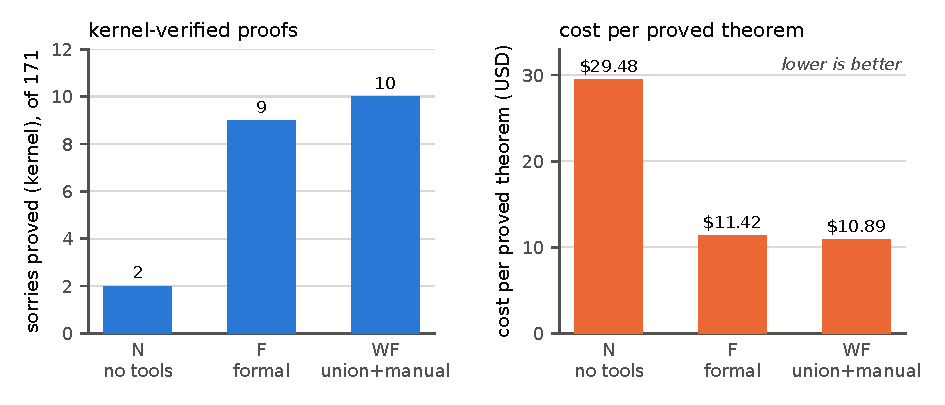
\includegraphics[width=\textwidth]{figures/fig4_sorrydb}
\caption{SorryDB, one-shot drafting with no compiler in the loop. Left:
kernel-verified proofs out of 171 live-pin tasks. Right: cost per proved
theorem --- tools raise total spend but \emph{cut} the cost of each success
by $2.7\times$. Data: \code{bench/v2/runs/sorrydb/verify.jsonl} $\times$
the run rows.}
\label{fig:sorrydb}
\end{figure}

\begin{figure}[htbp]
\centering
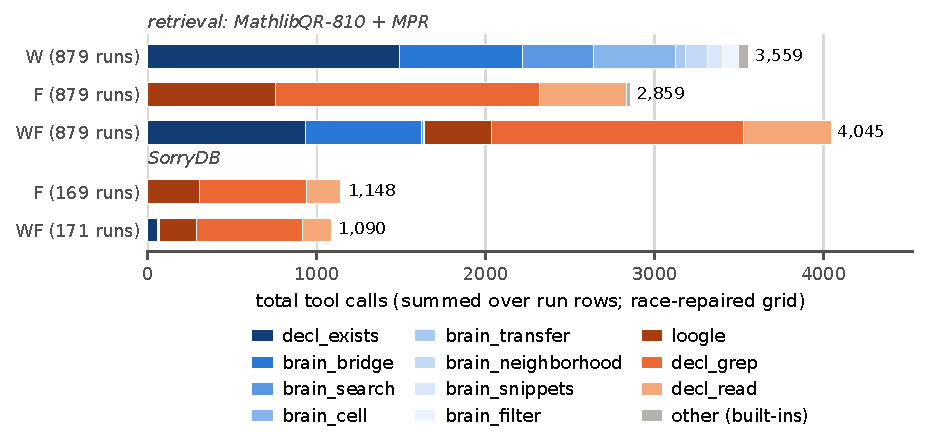
\includegraphics[width=\textwidth]{figures/fig5_tooluse}
\caption{Tool composition by arm: total calls summed over run rows
(retrieval pools QR-810 and MPR, 879 runs/arm; SorryDB ${\sim}$170
runs/arm). Blues are Brain tools, oranges formal-search tools, gray the
CLI's built-ins. \code{decl\_exists} dominates every Brain-bearing arm;
under the manual (WF) the Brain toolkit contracts to
\code{brain\_bridge}\,+\,\code{decl\_exists} (\code{brain\_cell}: 482 calls
in W, one in WF); and on SorryDB the WF agent routes 94\% of its calls to
formal search --- the concept $\neq$ premise boundary, visible in the
agents' own routing. Data: \code{transcript\_stats.tool\_calls\_by\_name}
summed over \code{bench/v2/runs/}.}
\label{fig:tooluse}
\end{figure}

Three notes complete the record. (i)~8 candidate proofs --- all from
curve25519-dalek-lean-verify, whose verification pass covered only 2 of its
10 candidates --- carry no kernel verdict in \code{verify.jsonl}; they are
conservatively counted as not-proved above. (ii)~3 (N) and 2 (F) tasks have
no run row at all (runner losses). (iii)~2 stale verdicts against dead-pin
rows from the first verification pass are excluded. Distinct sorries proved
across all arms: 13; N's proofs are a strict subset of both F's and WF's;
WF vs.\ F overlap 6, WF-only 4, F-only 3 --- no significance claim at this
$n$.

\paragraph{Reading.} Tools triple-to-quintuple the kernel-verified prove
rate and nearly triple the honest-abstention rate; N instead burns its
budget, with 70 of its 168 rows producing nothing, mostly 600\,s timeouts.
Cost-per-proved-theorem \emph{falls} by $2.7\times$ even as total tool
spend rises --- verification effort is cheaper than blind search. One
comparison caveat: the published SorryDB agentic best (${\approx}30\%$,
union 35.7\%) is not comparable, both because the task subset differs (ours
is weighted toward research-frontier repos: PNT+, a cryptographic
verification codebase, LeanAPAP) and because the protocol differs
materially (published agents iterate against the build; ours drafted
one-shot with no compiler in the loop).

\section{Synthesis}\label{sec:synthesis}

\paragraph{What the join adds.} Two things, both now measured twice. The
first is \emph{grounding}: binary existence verification at the
informal$\to$formal boundary collapses hallucinated citations
(5.9\%/6.8\% vs.\ 10--26\%; checked-and-cited-anyway 13\% vs.\ 30--35\%),
and the effect grows off-distribution, where memory fails. The second is
\emph{concept entry}: when the query is a description rather than a name
--- the fresh set, the special\_case query style --- the curated join finds
what lexical and type-pattern search cannot (42\% vs.\ 16--25\%; nDCG 0.523
vs.\ 0.384). The fresh-set McNemar ($p < 0.0001$) says the join itself, not
corpus access, carries this.

\paragraph{Where it does not.} Premise selection ranks by a different
signal than concept identity: W trails F by 18pp on MathlibMPR, exactly as
preregistered from TheoremGraph's negative transfer. And the API's
single-shot free-text entry is a label resolver (0.036 R@10 in system
mode); everything the agent arms recover, they recover by reformulating
against it. The agents vote the same way with their calls: given both
toolkits on SorryDB, WF routes 94\% of its tool calls to formal search
(Figure~\ref{fig:tooluse}).

\paragraph{The composition result.} The toolkits are complementary, and a
briefed agent composes them into the best rows we know of on both
third-party benchmarks (QR 0.885, MPR 0.557) --- on gold labels we did not
write. This is the Bridge thesis restated in retrieval form: the join
\emph{plus} the territory beats either alone.

\paragraph{API roadmap, derived.} Four items follow directly from the data.
First, a semantic statement-level index behind \code{brain\_bridge}: the
$0.036 \to 0.816$ single-shot/agent gap is an entry-point problem, not a
content problem. Second, \code{brain\_premises(goal\_state)}, a
premise-level ranking mode with a measured 18pp target (BRIDGE-ISSUES \#7).
Third, the eight pre-campaign API requirements (batch \code{decl\_exists},
signatures + imports per hit, generalization surfacing, honest abstention,
cursored neighborhoods, snapshot echo, the composite \code{brain\_bridge},
teaching tool descriptions) were implemented before the campaign and are
what the arms exercised. Fourth, the \code{AGENT\_MANUAL.md} pattern
itself: distilling measured tool behavior (${\sim}5{,}500$ logged calls)
into a briefing eliminated the dominant misuse mode (\code{brain\_cell}
$63\% \to {\sim}0$) and is the cheapest intervention in the whole study.

\paragraph{Cost economics.} In Tier-1 the bridge arm is cheaper \emph{and}
better than its tool-bearing competitors (\$0.121/task vs.\ C \$0.140, E
\$0.128, at +2--26pp success). Retrieval runs at \$0.08--0.21/query (QR)
and \$0.18--0.44/query (MPR). In proving, tool arms cut
cost-per-proved-theorem from \$29 to \$11 while raising the prove rate
$5\times$. Across all three phases, adding the join never made the task
more expensive per success.

\section{Limitations and threats to validity}\label{sec:limitations}

\begin{enumerate}
\item \textbf{One model per phase.} Tier-1 is Haiku-only (per-model run
  dirs were not keyed --- fixed in v2, where dirs are (benchmark, arm,
  model)-keyed) and v2 is Sonnet-only, so a bridge that only helps some
  capability band would not be distinguished. The preregistered two-model
  grid remains undone.
\item \textbf{Agent-vs-retriever comparability.} Our QR/MPR agent rows spend
  multi-call reasoning and verification per query; published retriever rows
  embed once. ``Above the published rows'' is a statement about achievable
  quality at agent cost, not a same-budget comparison. System-mode is the
  same-budget comparison, and it loses badly.
\item \textbf{The WF manual confound.} WF bundles tool union with the
  briefing; the ablation exists in the harness but was not run.
\item \textbf{Power on secondary contrasts.} F-vs-W on QR is a null at
  $n=810$ ($p=0.36$); MPR has $n=69$; SorryDB proved counts are single
  digits per arm --- overlap patterns there are descriptive only.
\item \textbf{The judge leg was dropped, not repaired.} The preregistered
  faithful@budget metric (BEq+ equivalence) was never graded: the judge
  required human calibration (deviation 5), Jack's arm-correlated-bias
  critique stood, and the field precedent (TheoremGraph rejecting its own
  judge as over-generous) argued against resting headline claims on one.
  The v2 replacement --- graders that predate the arms --- is stronger, but
  it means Tier-1 ``success'' can still reward a well-formed wrong
  statement; the Tier-1 fresh-set numbers are best read jointly with the
  hallucination and trace evidence.
\item \textbf{Tier-1a is contaminated by construction} (arm A: 59.6\%); we
  report it for the paired deltas and as the memorization control against
  Tier-1b, never alone.
\item \textbf{SorryDB caveats.} One-shot drafting without a compiler
  under-represents every arm relative to published loops; the subset is
  repo-sampled, not difficulty-matched; 8 candidates lack verdicts; and
  45\% snapshot rot means the \emph{original} frozen subset is already
  partly unreproducible upstream --- the preserved
  \code{tasks\_frozen.jsonl} (goal states + context windows) is the durable
  record.
\item \textbf{Mechanical extractors.} Cited-declaration extraction is a
  documented regex heuristic; hallucination rates are comparable across
  arms (same extractor) but not exact.
\end{enumerate}

\section{Data availability}\label{sec:data}

{\sloppy
Everything needed to recompute this report lives in the private preservation
repository \textbf{\code{Deicyde/wikilean-bridge-experiment}} (report at the
root as \code{README.md} and under \code{report/}). Provenance commits refer
to the WikiLean working repository. See Table~\ref{tab:files}.\par}

\begin{table}[htbp]
\centering
\footnotesize
\begin{tabular}{@{}p{0.34\textwidth}p{0.40\textwidth}p{0.18\textwidth}@{}}
\toprule
Path (preservation repo) & Contents & Key provenance commits (WikiLean) \\
\midrule
\code{docs/research/BRIDGE-EXPERIMENT.md} & preregistration incl.\ deviations 1--7 & \code{0d36f266} (2026-07-16) \\
\code{docs/research/BRIDGE-RESULTS.md} & Tier-1 + retrieval results log & \code{53f5cb31}, \code{daac6107} \\
\code{docs/research/BRIDGE-V2-BENCHMARKS.md} & v2 design + verified sources & --- \\
\code{docs/research/BRIDGE-ISSUES.md} & issue queue / history & \code{cdc2d743} \\
\code{bench/*.py}, \code{bench/README.md}, \code{bench/arms/} & Tier-1 harness: runner, scorer, REPL typecheck rig, trace analysis, arm manifests & \code{068abe34}, \code{e554902e}, \code{6c2ca704}, \code{31b95caa}, \code{79ac3dfe} \\
\code{bench/data/bridge\_tasks.jsonl} (+\code{.stats}) & 371 ProofNet\# tasks; source pin + MIT licence in stats & \code{e554902e}, \code{ec2a9e11} \\
\code{bench/data/fresh\_tasks.jsonl} (+\code{.stats}) & 100 fresh tasks + determinacy annotations + held-out guarantee & \code{df5dbf92}, \code{a0d45103} \\
\code{bench/data/gold\_census.json}, \code{fresh\_census.json} & which golds elaborate on which pin; fresh pin = Lean v4.33.0-rc1 / Mathlib \code{9944fe29} (Tier-1a pin = v4.32.0-rc1 / \code{a33a5ccd}, recorded in \code{bench/README.md}) & \code{01e8612b}, \code{185377cc} \\
\code{bench/data/bridge\_summary.json} & Tier-1 scored summary: per-arm aggregates, paired matrix, McNemar tables & \code{53f5cb31} \\
\code{bench/data/runs/} & all 2{,}355 Tier-1 run rows (5 arms $\times$ 471) & --- \\
\code{bench/data/runs\_devleak\_2026-07-18/} & the 120 quarantined skill-leak dev runs (deviation 6 evidence) & \code{f89e7a41} \\
\code{bench/v2/} & v2 harness + \code{AGENT\_MANUAL.md} & \code{c7629584}, \code{21032c06} \\
\code{bench/v2/data/} & MathlibQR/MPR (LeanSearch-v2 @\code{94f4888cbaf9}, CC BY 4.0), SorryDB-2601 split, \code{tasks\_frozen.jsonl} & \code{c7629584}, \code{87638cfc}, \code{db679e8d} \\
\code{bench/v2/runs/} & every v2 run row \textbf{with full gzipped stream-json transcripts} (QR 810$\times$4, MPR 69$\times$4, SorryDB 508 rows) + \code{verify.jsonl} (197 kernel verdicts) & \code{3664aa3d}, \code{daac6107}, \code{382e51bf}, \code{1fe21cca} \\
\bottomrule
\end{tabular}
\caption{File map of the preservation repository.}
\label{tab:files}
\end{table}

Recomputation entry points: \code{bench/score\_bridge.py} (Tier-1),
\code{bench/trace\_analysis.py} (Section~\ref{sec:trace}),
\code{bench/v2/score\_retrieval.py} (Section~\ref{sec:retrieval} ---
reprints every table), \code{bench/v2/verify\_sorrydb.py}
(Section~\ref{sec:sorrydb} verdicts; the Table~\ref{tab:sorrydb} rows are a
straight aggregation of \code{verify.jsonl} $\times$ the run rows, filtered
to \code{tasks\_frozen.jsonl} ids, counting \code{gave\_up}, \code{error},
verdicts, and \code{transcript\_stats.cost\_usd}). The figures in this
document are generated from those same files by
\code{report/bridge-report/recompute\_figdata.py} (which asserts every
plotted value against the markdown report) and
\code{generate\_figures.py}.

External sources cited (all fetched and verified during the v2 design
sweep): TheoremGraph~\cite{theoremgraph} $\cdot$
LeanSearch~\cite{leansearch} $\cdot$ LeanSearch-v2~\cite{leansearchv2}
$\cdot$ LeanExplore~\cite{leanexplore} $\cdot$ SorryDB~\cite{sorrydb}
$\cdot$ FATE~\cite{fate} $\cdot$ miniCTX~\cite{minictx} $\cdot$
LeanDojo~\cite{leandojo} $\cdot$ LeanAgent~\cite{leanagent} $\cdot$
Numina-Lean-Agent~\cite{numina} $\cdot$ miniF2F-v2~\cite{minif2fv2} $\cdot$
ProofNet\#/ProofNetVerif~\cite{proofnetsharp} $\cdot$ benchmark-faults
survey~\cite{benchfaults}.

\appendix

\section{The agent tool manual}\label{app:manual}

{\itshape What follows is \code{bench/v2/AGENT\_MANUAL.md}, the briefing
prepended verbatim to every WF-arm prompt --- it is part of the measured
condition (Section~\ref{sec:retrieval}) and is reproduced here unchanged
as a study artifact.}

\subsection*{Tool manual: searching Mathlib with the Brain + formal search}

You have two complementary toolkits. Every claim in this manual is measured
from ${\sim}5{,}500$ logged tool calls across 3{,}500 benchmark runs
(Tier-1 + Bridge v2); numbers in brackets are those measurements.

\subsection{The mental model}

\begin{itemize}
\item \textbf{The Brain (wikibrain, 8 tools)} is a \emph{curated knowledge
  graph} joining informal mathematics (Wikipedia/Wikidata concepts,
  external databases) to Mathlib declarations. It knows what things
  \emph{mean} and how concepts relate --- but it only ``atomizes''
  declarations that some concept, annotation, or tag claims (${\sim}$12k of
  Mathlib's declarations). It is a map, not the territory.
\item \textbf{Formal search (3 tools)} operates on \emph{all} of Mathlib
  directly: type-pattern search (loogle), source grep, source reading. It
  knows everything that exists but nothing about what it means informally.
\end{itemize}

Rule of thumb: \textbf{route by what you're holding.} Holding a concept
described in words $\to$ start with the Brain. Holding a type shape or name
fragment $\to$ start with formal search. Always finish with
\code{decl\_exists} on every name you intend to output.

\subsection{Formal search tools}

\subsubsection{\code{loogle}}
Type-pattern and constant search (the public \code{loogle.lean-lang.org}
service).
\begin{itemize}
\item USE for: ``a lemma whose statement looks like
  \code{\_ * \_ ${\leq}$ \_ * \_}'', searches by involved constants
  (\code{Real.sqrt}, \code{tsum}), name substrings.
\item Strengths: covers ALL of Mathlib; ${\sim}$0\% call errors [578 calls,
  0 errors]; the best premise-finding tool --- the loogle+grep toolkit
  matched a specialist premise retriever [group-recall@10 0.453 vs 0.461
  SOTA].
\item Weaknesses: needs Lean syntax fluency; a wrong pattern silently
  returns unrelated hits; small result payloads mean you often need
  decl\_read next.
\end{itemize}

\subsubsection{\code{decl\_grep}}
Regex search over the Mathlib source checkout (ripgrep).
\begin{itemize}
\item USE for: name fragments (``cantor''), notation, docstring phrases,
  finding the file a declaration lives in.
\item Strengths: the workhorse [1{,}206 calls, 0\% errors]; catches things
  loogle's type index can't (comments, docstrings, naming conventions).
\item Weaknesses: lexical only --- if the concept's name doesn't appear in
  source, grep cannot find it (descriptive queries like ``special case of
  X'' score worst for grep-based agents [nDCG 0.384 vs the Brain's 0.523]).
\end{itemize}

\subsubsection{\code{decl\_read}}
Read declaration source (with surrounding context) from the checkout.
\begin{itemize}
\item USE for: verifying a candidate actually says what you think BEFORE
  citing it; getting exact signatures and hypotheses.
\item Strengths: ground truth for any decl in Mathlib [397 calls, 0\%
  errors].
\item Weaknesses: you need the file/name first --- it is a confirmation
  tool, not a discovery tool.
\end{itemize}

\subsection{Brain tools}

\subsubsection{\code{brain\_bridge} --- THE ENTRY POINT for
informal$\to$formal}
Free text in, existence-verified declarations + owning atoms out, with
signatures, import lines, and one-hop dependency context.
\begin{itemize}
\item USE for: ``the concept described as $\langle$words$\rangle$'' ---
  especially nicknames and special-case descriptions, where the Brain's
  curated bonds beat grep [special\_case nDCG 0.523 vs 0.384; nickname
  0.779 vs 0.757].
\item CRITICAL LIMITATION (measured): its free-text matching is
  label/alias anchored, NOT semantic. A single call with a descriptive
  paraphrase usually misses [single-shot benchmark: 3.6\% R@10 vs 82\% for
  an agent that reformulates]. \textbf{Never accept one miss as the answer:
  reformulate 2--4 times} --- try the concept's canonical name, a synonym,
  the head noun alone. 8.9\% of calls return \code{match:"none"} [727
  calls]; that response includes nearest-candidate suggestions --- read
  them.
\item The \code{hits} list is existence-verified; bond quality matters:
  \code{exact} means the decl IS the concept; \code{formalizes}/weaker
  bonds are nearby.
\end{itemize}

\subsubsection{\code{brain\_search}}
Fuzzy label + alias search returning atoms (cells).
\begin{itemize}
\item USE for: resolving a name you half-know into an atom id; browsing
  what the Brain calls something [400 calls, 0\% errors --- the reliable
  fallback when brain\_bridge misses].
\item Weaknesses: returns atoms, not ranked decls --- follow with
  brain\_cell on the winning atom.
\end{itemize}

\subsubsection{\code{brain\_cell}}
The full atom card: Lean code, Wikidata description, DB snippets, organs.
\begin{itemize}
\item USE for: everything known about ONE object after bridge/search
  resolved it.
\item \textbf{THE \#1 MISUSE [63\% of 482 calls failed]: calling it with a
  bare \code{decl:Mathlib:Name} for an arbitrary declaration.} The Brain
  only has atoms for concept-joined decls; ``unresolvable key'' means
  \emph{no atom owns this decl}, NOT that the decl doesn't exist. For
  arbitrary decls use decl\_exists (works for all of Mathlib) and
  decl\_read for source. Call brain\_cell only with ids that came OUT of a
  Brain tool.
\end{itemize}

\subsubsection{\code{decl\_exists} --- THE DISCIPLINE TOOL}
Batch existence check for declaration names (backed by the full oracle ---
covers ALL of Mathlib, unlike brain\_cell).
\begin{itemize}
\item \textbf{USE ALWAYS, on every name you are about to output.} This is
  the measured difference between grounded and hallucinated citations:
  agents that verified before citing cut hallucinated-but-cited-anyway to
  13\% vs 33\% for agents relying on fuzzy search results alone. It is
  cheap [1{,}473 calls, 0.1\% errors] and batched --- check 10 names in one
  call.
\item Also returns verified-rename suggestions for stale names.
\end{itemize}

\subsubsection{\code{brain\_neighborhood}}
The synapse graph around an atom (depends/links/relates, cursored).
\begin{itemize}
\item USE for: ``what connects to X'' --- finding the connecting lemma
  between two concepts, walking dependencies.
\item Weaknesses: needs a valid atom id [24.8\% of calls errored --- same
  unresolvable-key trap as brain\_cell; resolve the atom first].
\end{itemize}

\subsubsection{\code{brain\_transfer} / \code{brain\_snippets} /
\code{brain\_filter}}
Narrower tools: label$\leftrightarrow$decl jumps for KNOWN labels
(transfer), stored source snippets (snippets), facet enumeration (filter).
High misuse rates when fed non-atom ids [40\%/57\% errors]. Prefer
brain\_bridge/brain\_search entry; reach for these only on ids the Brain
already returned.

\subsection{Routing playbook}

\begin{center}
\small
\begin{tabular}{@{}p{0.30\textwidth}p{0.62\textwidth}@{}}
\toprule
You are holding & Do this \\
\midrule
A concept in words & brain\_bridge $\to$ (miss?) reformulate $\to$
  brain\_search $\to$ brain\_cell \\
A special case / nickname & brain\_bridge (the Brain's best terrain) \\
A type shape & loogle \\
A name fragment & decl\_grep \\
Premises for a proof & loogle + decl\_grep FIRST [0.453 vs 0.272], Brain
  for concept grounding \\
A candidate name to cite & decl\_exists (batch, always) $\to$ decl\_read
  if the statement matters \\
An atom id from any Brain tool & brain\_cell / brain\_neighborhood freely \\
A bare decl name needing info & decl\_exists + decl\_read --- NOT
  brain\_cell \\
\bottomrule
\end{tabular}
\end{center}

\subsection{Anti-patterns (each one measured in prior runs)}

\begin{enumerate}
\item \textbf{Citing unverified names.} 33\% of hallucinated citations came
  from agents that had search evidence in front of them and cited a wrong
  name anyway. decl\_exists is binary and kills this.
\item \textbf{One query, then giving up.} The single-call miss rate on
  descriptive queries is ${\sim}$96\%; agents that reformulate reach
  ${\sim}$82\%. Iteration IS the algorithm.
\item \textbf{brain\_cell as a generic decl inspector.} 63\% failure rate.
  Brain atoms $\neq$ all of Mathlib.
\item \textbf{Answering outside the requested format.} 143/810 no-tool runs
  were scored 0 for exactly this. Re-read the output contract before
  replying.
\item \textbf{Inventing tool names} (e.g.\ \code{logue}, \code{lookie}).
  Use the names above.
\end{enumerate}

\begin{thebibliography}{13}
\itemsep2pt

\bibitem{theoremgraph}
TheoremGraph. arXiv:2606.25363.
\url{https://arxiv.org/abs/2606.25363}

\bibitem{leansearch}
LeanSearch. arXiv:2403.13310.
\url{https://arxiv.org/abs/2403.13310}

\bibitem{leansearchv2}
LeanSearch-v2. arXiv:2605.13137. Data: pinned
\code{frenzymath/LeanSearch-v2} @\code{94f4888cbaf9}, CC BY 4.0.
\url{https://arxiv.org/abs/2605.13137};
\url{https://github.com/frenzymath/LeanSearch-v2}

\bibitem{leanexplore}
LeanExplore. arXiv:2506.11085.
\url{https://arxiv.org/abs/2506.11085}

\bibitem{sorrydb}
SorryDB. arXiv:2603.02668.
\url{https://arxiv.org/abs/2603.02668};
\url{https://sorrydb.org}

\bibitem{fate}
FATE. arXiv:2511.02872.
\url{https://arxiv.org/abs/2511.02872}

\bibitem{minictx}
miniCTX. arXiv:2408.03350.
\url{https://arxiv.org/abs/2408.03350}

\bibitem{leandojo}
LeanDojo. arXiv:2306.15626.
\url{https://arxiv.org/abs/2306.15626}

\bibitem{leanagent}
LeanAgent. arXiv:2410.06209.
\url{https://arxiv.org/abs/2410.06209}

\bibitem{numina}
Numina-Lean-Agent. arXiv:2601.14027.
\url{https://arxiv.org/abs/2601.14027}

\bibitem{minif2fv2}
miniF2F-v2. arXiv:2511.03108.
\url{https://arxiv.org/abs/2511.03108}

\bibitem{proofnetsharp}
ProofNet\#/ProofNetVerif. arXiv:2406.07222. Tasks pinned to
\code{PAug/ProofNetSharp} @\code{a8da405f} (MIT).
\url{https://arxiv.org/abs/2406.07222}

\bibitem{benchfaults}
Benchmark-faults survey. arXiv:2606.29493.
\url{https://arxiv.org/abs/2606.29493}

\end{thebibliography}

\end{document}
